\documentclass[a4paper,11pt,exos]{nsi} % COMPILE WITH DRAFT


\begin{document}
\classe{\terminale Comp}
\titre{Population de cigognes}
\maketitle

Une population est un groupe d'individus appartenant à une même espèce et vivant dans une zone définie.\\
Les écologistes s'efforcent de comprendre les causes de la variation de la taille des populations et de prédire les tendances de ces nombres dans le temps et d'un endroit à l'autre.\\
La taille d'une population augmente grâce aux naissances et à l'immigration d'individus de l'extérieur. Les décès et l'émigration diminuent la taille de la population.\\
Ces entrées et sorties peuvent être représentées sous la forme d'une équation où l'indice $t$ indique un moment discret dans le temps.

\begin{center}
  \begin{minipage}[c]{.65\linewidth}
La population alsacienne de cigognes blanches (\emph{ciconia ciconia}), en déclin à partir de la fin des années 1950, comme toutes les populations de l'Ouest européen, a fait l'objet de dénombrements très sûrs, compte-tenu de la rareté de l'espèce et de la facilité de son
observation.
   \end{minipage} \hfill
   \begin{minipage}[c]{.3\linewidth}
\begin{center}
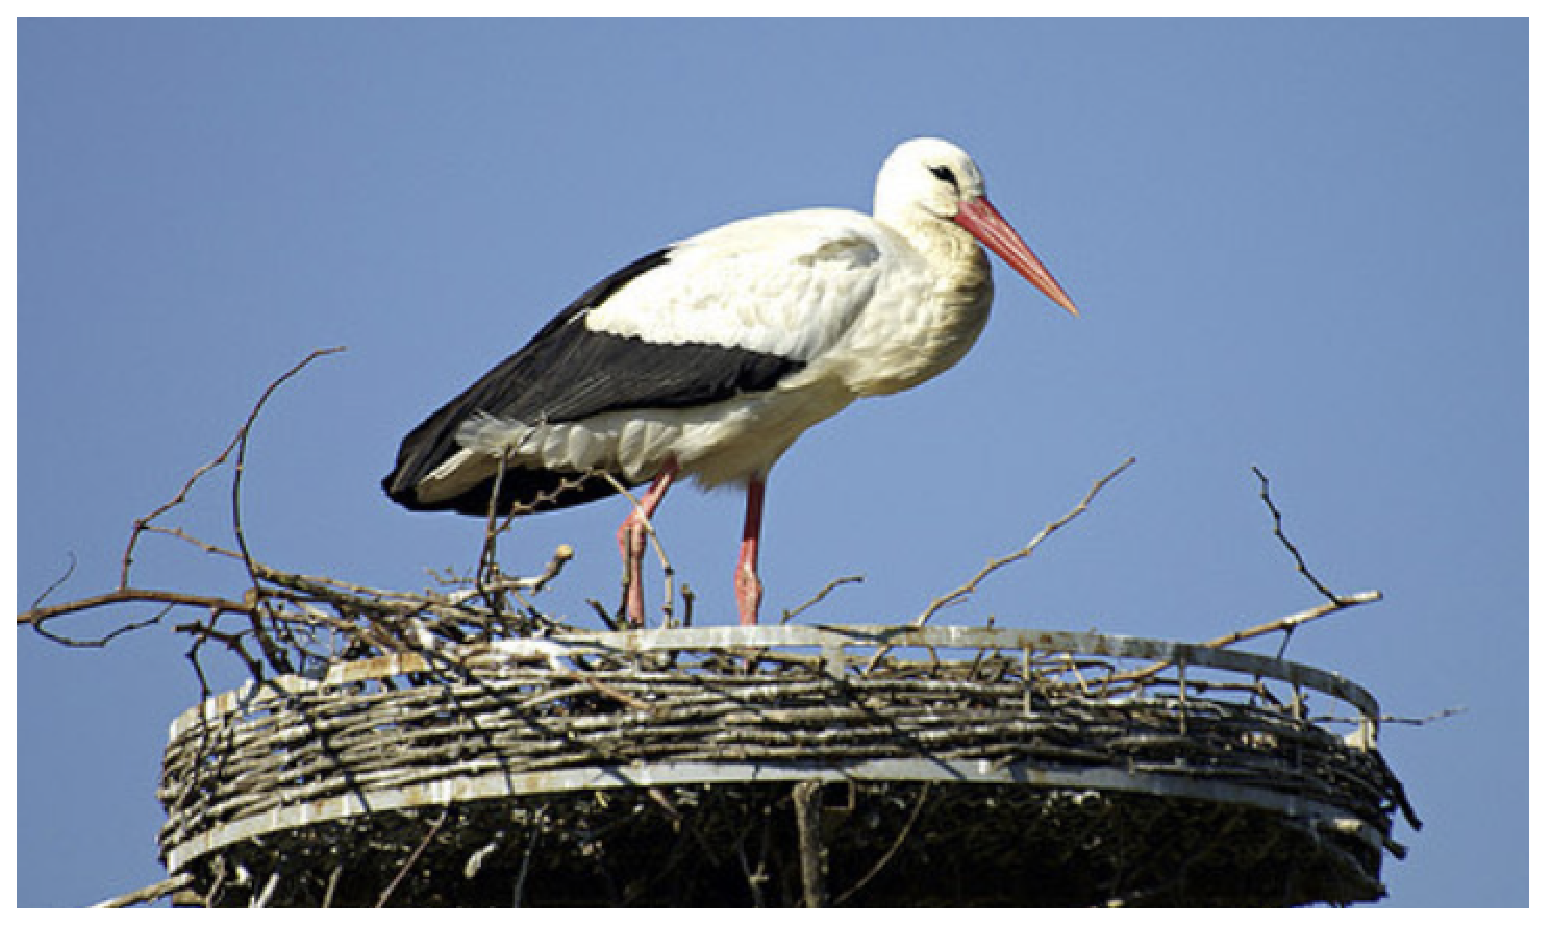
\includegraphics[scale=0.2]{cigogne.eps} 
\end{center}
   \end{minipage}
\end{center}

On dispose donc d'excellentes données dues à Schierer (1972).
Durant la période 1960-70 le nombre de couples nicheurs de cette population a évolué de
la manière suivante.
\begin{center}
    \tabstyle[UGLiBlue]
\begin{tabular}{|l|c|c|c|c|c|c|c|c|c|c|c|}
\hline
\ccell Année &1960 & 1961 & 1962 & 1963 & 1964 & 1965 & 1966 & 1967 & 1968 & 1969 & 1970 \\\hline
\ccell Effectifs &145 & 117 & 90 & 80 & 67 & 54 & 58 & 39 & 42 & 23 & 23 \\\hline
\end{tabular}
\end{center}


\textbf{Le but de l'activité est de modéliser l'évolution de la population des cigognes.}

\section*{Partie A - Étude graphique}
\begin{enumerate}
    \item Représenter le nuage de points dans le repère ci dessous. (On n'oubliera pas d'indiquer la légende)
    \begin{center}
    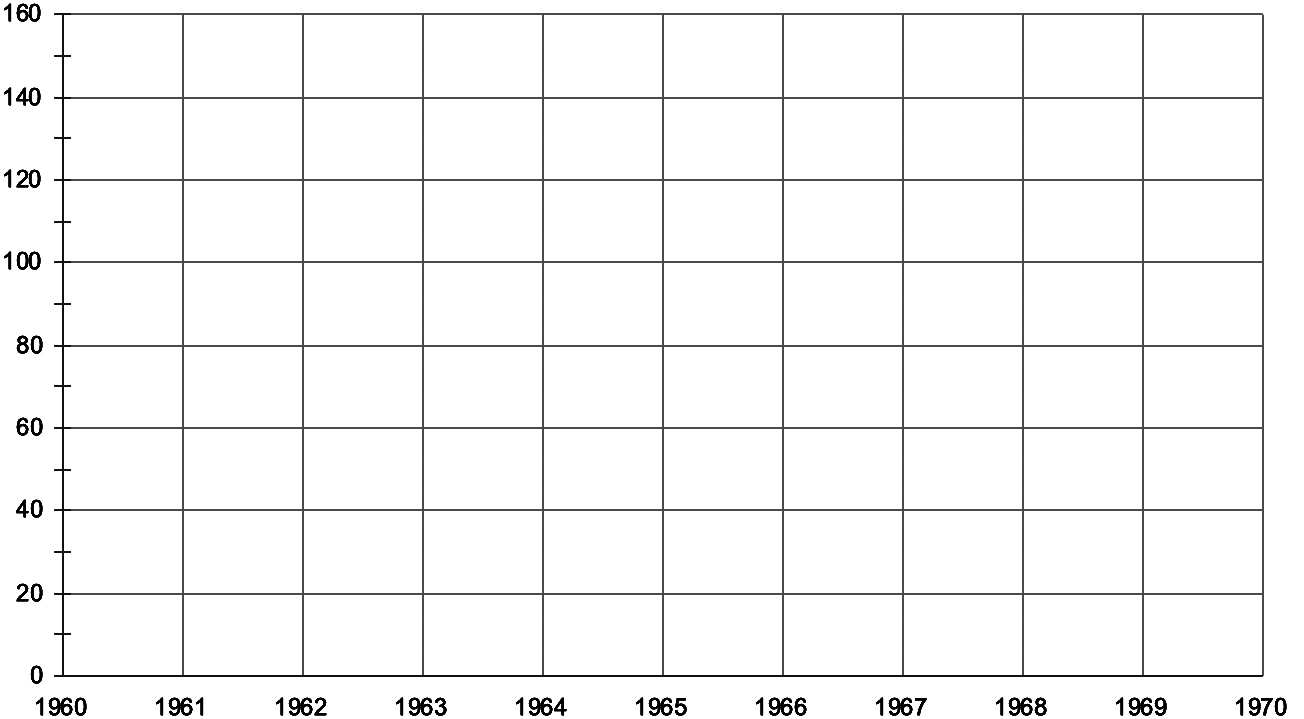
\includegraphics[width=12cm]{repere.png} 
    \end{center}
    \item Décrire ce nuage de points (évolution, tendance).\\[.5em]
    \carreauxseyes{16}{1.6}
\end{enumerate}

\section*{Partie B - Modélisation par une suite}
On considère donc la population de cigognes composée de 145 couples d'individus.\\
Pour tout entier naturel $n$, on note $u_n$ le nombre de couples de cigognes au bout de $n$ années. Ainsi on a $u_0=145$.
\begin{enumerate}
    \item La suite $(u_n)$ est-elle arithmétique ? géométrique ?
    \item On propose  d’approcher les valeurs de la suite $(u_n)$ par \textbf{une suite arithmétique $(v_n)$}.
    \begin{enumalph}
        \item Compléter le tableau suivant :\\[.5em]
        %\begin{center}
            \tabstyle[UGLiBlue]
        \begin{tabular}{|m{2.6cm}|c|c|c|c|c|c|c|c|c|c|c|}
        \hline
        \ccell Année &1960 & 1961 & 1962 & 1963 & 1964 & 1965 & 1966 & 1967 & 1968 & 1969 & 1970 \\\hline
        \ccell Effectifs & 145 & 117 & 90 & 80 & 67 & 54 & 58 & 39 & 42 & 23 & 23 \\\hline
        \ccell \small Différence entre deux valeurs consécutives &\ccell & & & & & & & & & & \\\hline
        \end{tabular}
        \vspace*{.2cm}
        %\end{center}
        \item À l'aide du tableau complété, proposer une raison pour cette suite arithmétique $(v_n)$.
        \item  Exprimer $v_n$ en fonction de $n$ pour tout entier naturel $n$.\\ Représenter la suite $(v_n)$ dans le repère précédent.
    \end{enumalph}
    \item On propose maintenant d’approcher les valeurs de la suite $(u_n)$ par une \textbf{suite géométrique $(w_n)$}.
    \begin{enumalph}
        \item Compléter le tableau suivant :\\[.5em]
        %\begin{center}
            \tabstyle[UGLiBlue]
        \begin{tabular}{|m{2.6cm}|c|c|c|c|c|c|c|c|c|c|c|}
        \hline
        \ccell Année &1960 & 1961 & 1962 & 1963 & 1964 & 1965 & 1966 & 1967 & 1968 & 1969 & 1970 \\\hline
        \ccell Effectifs & 145 & 117 & 90 & 80 & 67 & 54 & 58 & 39 & 42 & 23 & 23 \\\hline
        \ccell \small Quotient de deux valeurs consécutives &\ccell & & & & & & & & & & \\\hline
        \end{tabular}
        %\end{center}
        \vspace*{.2cm}
        \item À l'aide du tableau complété, proposer une raison pour cette suite géométrique $(w_n)$.
        \item  Exprimer $w_n$ en fonction de $n$ pour tout entier naturel $n$.\\ Représenter la suite $(w_n)$ dans le repère précédent.
    \end{enumalph}
    \item  Lequel des deux modèles est-il préférable de conserver ?
    
    \item Dans la suite, on prendra  0,848 comme raison de la suite géométrique $(w_n)$.\\
    \begin{minipage}[c]{.55\linewidth}
        On souhaite utiliser un algorithme afin de déterminer l’année
        d’extinction de l’espèce. \\
        On considère  que cette espèce est éteinte lorsque le nombre de couples est inférieur à 5.
        \begin{enumalph}
            \item Compléter l’algorithme ci-contre afin qu’il répondre au problème.
            \item Déterminer la date théorique à laquelle cette population s’est  
            éteinte.
        \end{enumalph}
    \end{minipage}
    \hspace*{.5cm}
    \begin{minipage}[c]{.4\linewidth}
        \begin{pyc}
            \begin{minted}{python}
                def extinction() :
                    u = ...
                    n = ...
                    while .......... :
                        n = n+1
                        u = ...
                    return ...
            \end{minted}
        \end{pyc}
    \end{minipage}
\end{enumerate}

\section*{Du discret au continu}
Pour modéliser une situation, on peut utiliser un modèle discret (avec des suites) comme dans la partie B, ou continu (avec une fonction). Ainsi, à partir d’un nuage de points, on essaie de trouver une courbe de tendance qui ajustera au mieux le nuage de points. L’équation de la courbe de tendance nous donne la fonction modélisant notre population.
\begin{enumerate}
    \item Nous allons utiliser GéoGebra pour déterminer la courbe de tendance la plus adaptée au nuage de points. Pour cela :
    \begin{enumerate}[label=\textbullet]
        \item Ouvrir l'activité Capytale n°9eca-3819455.
        \item Sélectionner les valeurs. Cliquer sur « statistiques à
        deux variables ».
        \begin{center}
            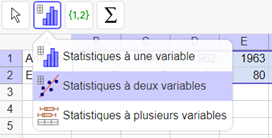
\includegraphics[width=5cm]{geogebra1.png}
        \end{center}
        \item Le nuage de points s'affiche. Dans « modèle d’ajustement » : choisir dans le menu déroulant le modèle le plus adapté.
        \begin{center}
            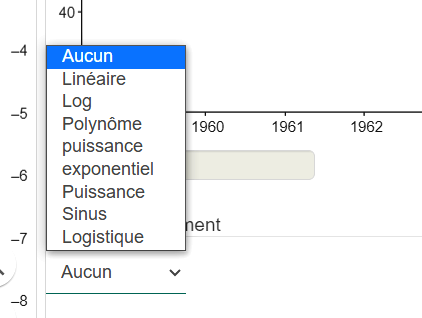
\includegraphics[width=5cm]{geogebra2.png}
        \end{center}
    \end{enumerate}

    \item Le modèle continu permet d'estimer la taille de la population de cigognes à différente date.
    \begin{center}
    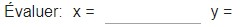
\includegraphics[width=5cm]{geogebra3.jpg}
    \end{center}
    \begin{enumalph}
        \item Quelle estimation du nombre de couples de cigognes en juin 1962 peut-on donner ?\\[.5em]
        \carreauxseyes{16}{1.6}
        \item Déterminer la date théorique à laquelle cette population s’est éteinte avec le modèle que vous avez choisi.\\[.5em]
        \carreauxseyes{16}{1.6}
    \end{enumalph}
\end{enumerate}
\end{document}